\documentclass{beamer}

\mode<presentation> {
\usetheme{Madrid}
}

\usepackage{graphicx} 
\usepackage{booktabs} 
\usepackage[utf8]{inputenc}
\newtheorem{thm}{Theorem}
\newtheorem{pf}{Proof}
\newtheorem{df}{Definition}

%%%%%%%%%%%%%%%%%%%%%%%%%%%%%%%%%%%%%%%%%%%%%%%%%%%%%%%%%%%%%%%%%%%%%%%%
%%%%%%%%%%%%%%%%%%%%  TITLE PAGE  %%%%%%%%%%%%%%%%%%%%%%%%%%%%%%%%%%%%%%  %%%%%%%%%%%%%%%%%%%%%%%%%%%%%%%%%%%%%%%%%%%%%%%%%%%%%%%%%%%%%%%%%%%%%%%%
\title{Dependence modelling using copulas}
\author{Edyta Pietrucha}

\date{\today}

%%%%%%%%%%%%%%%%%%%%%%%%%%%%%%%%%%%%%%%%%%%%%%%%%%%%%%%%%%%%%%%%%%%%%%%%
\begin{document}
\begin{frame}
\titlepage 
\end{frame}

\begin{frame}{Subject of analysis}

\fontsize{10}{13}\selectfont
Objective: Modelling dependency structure between stock indexes from three sectors:
\begin{itemize}
    \item Information technology: Apple (AAPL), Microsoft (MSFT), Nvidia (NVDA),
    \item Finance: Citigroup Inc (C), Goldman Sachs Group Inc (GS), JPMorgan Chase \& Co (JPM),
    \item Services: The Walt Disney Company (DIS), Netflix (NFLX), Amazon.com (AMZN).
\end{itemize}
Data: Daily values on close from 2014/08/25 to 2022/08/23. \\
Metrics: AIC, BIC, Log-likelihood. \\
Conclusion: 
\begin{itemize}
    \item Marginals -- best metrics scores achived for t-Student distribution.
    \item Joint distribution -- best metrics scores achived for D-vine copula.
\end{itemize}
    
\end{frame}

\begin{frame}{Indexes}

\centering
\begin{figure}[!h]
  \centering
    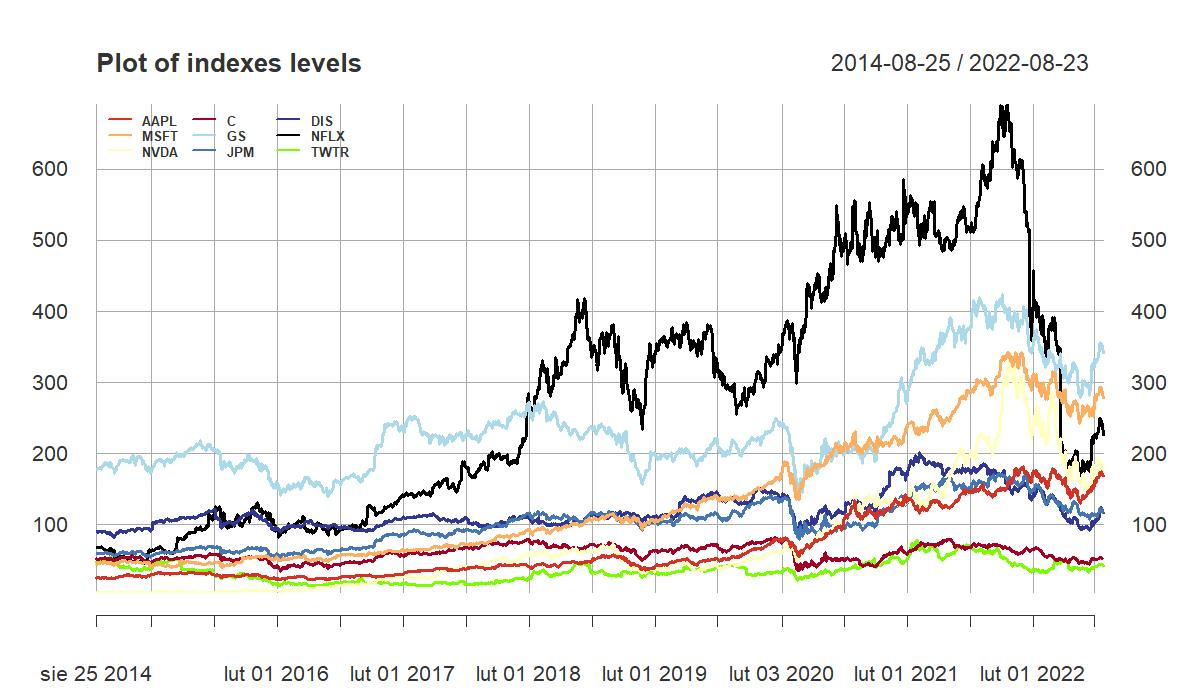
\includegraphics[width=1\textwidth]{figures/indexes_lvls.jpeg}
\end{figure}
    
\end{frame}

\begin{frame}{Spearman correlation matrix}
\centering
\begin{figure}[!h]
  \centering
    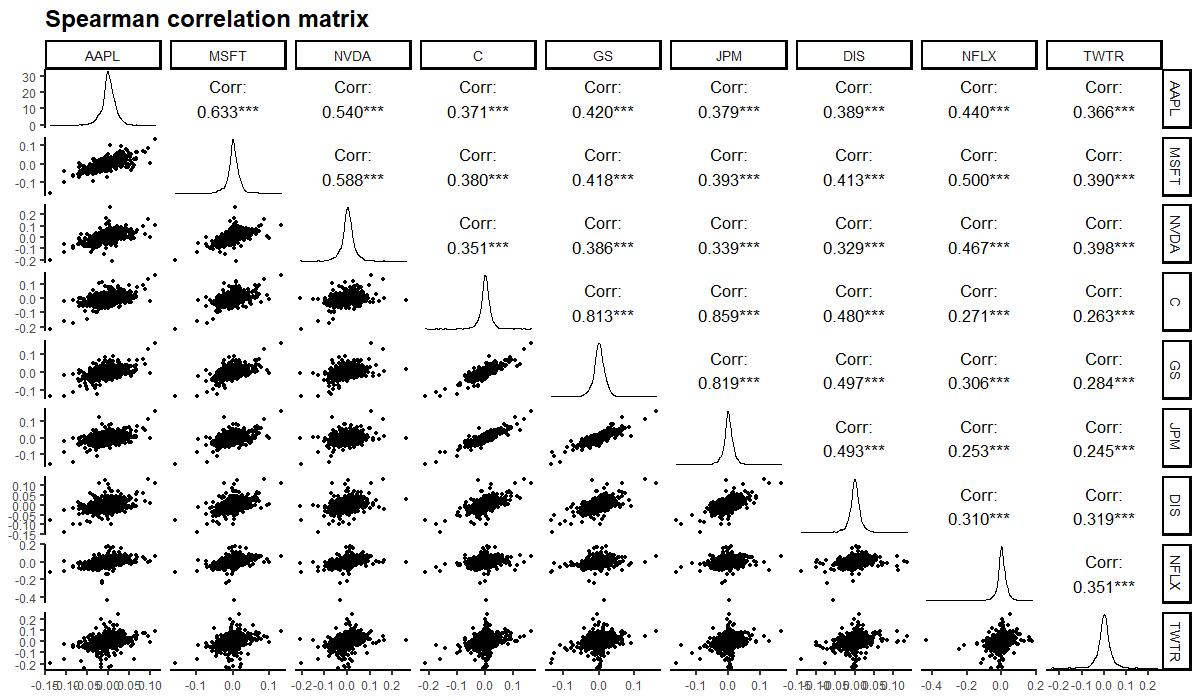
\includegraphics[width=1\textwidth]{figures/correlation/spearman_matrix.jpeg}
\end{figure}
    
\end{frame}

\begin{frame}{Histogram of logarithmic increments}

\centering
\begin{figure}[!h]
  \centering
    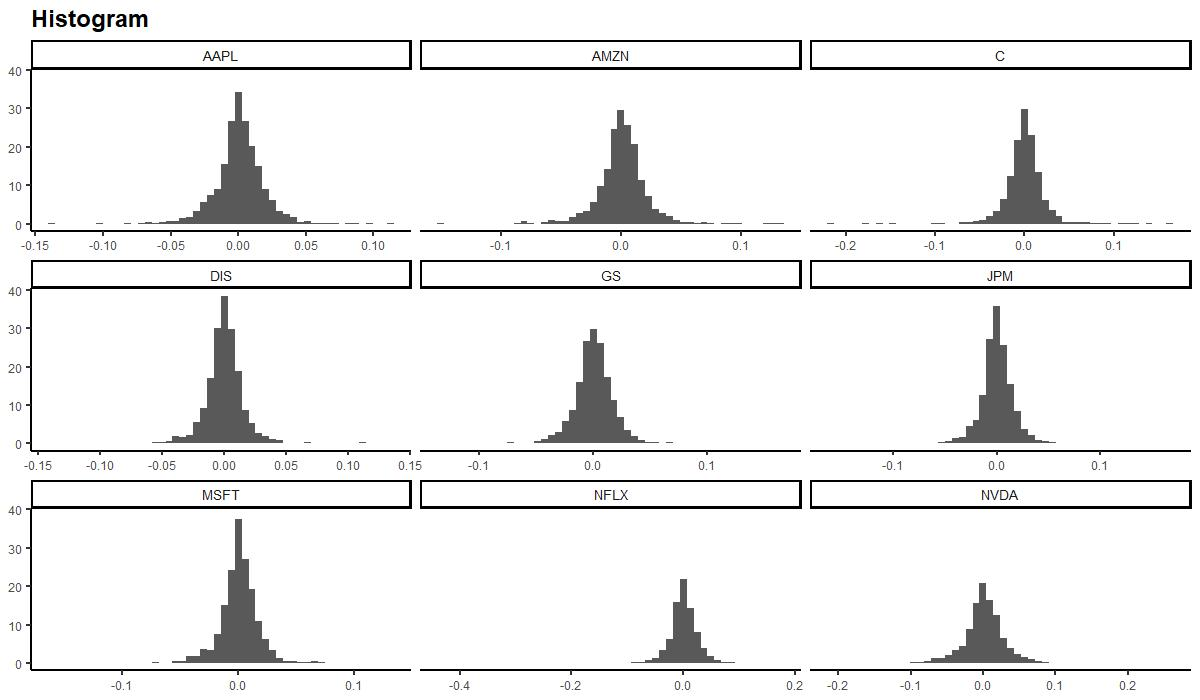
\includegraphics[width=1\textwidth]{figures/histogram_indexes.jpeg}
\end{figure}
    
\end{frame}

\begin{frame}{AIC for fitted marginals}

\centering
\begin{table}
\begin{table}[H]

\caption{AIC scores for fitted marginals.}
\centering
\fontsize{11}{13}\selectfont
\begin{tabular}[t]{lrrrr}
\toprule
Ticker & Gaussian & t-Student & Cauchy & Logistic\\
\midrule
AAPL & -10371.47 & -10734.44 & -10412.40 & -10658.04\\
MSFT & -10633.29 & -11042.11 & -10809.60 & -11003.79\\
NVDA & -8505.15 & -8908.12 & -8594.30 & -8821.99\\
C & -9744.16 & -10462.98 & -10177.07 & -10277.89\\
GS & -10338.31 & -10785.15 & -10406.27 & -10701.03\\
JPM & -10515.94 & -11123.16 & -10822.05 & -10981.67\\
DIS & -10691.22 & -11326.85 & -11118.12 & -11198.80\\
NFLX & -8554.29 & -9263.09 & -8945.58 & -9115.93\\
AMZN & -9977.81 & -10450.31 & -10149.33 & -10331.41\\
\bottomrule
\end{tabular}
\end{table}
   
\end{table}

\end{frame}

\begin{frame}{BIC for fitted marginals}

\centering
\begin{table}
\begin{table}[H]

\caption{BIC scores for fitted marginals.}
\centering
\fontsize{11}{13}\selectfont
\begin{tabular}[t]{lrrrr}
\toprule
Ticker & Gaussian & t-Student & Cauchy & Logistic\\
\midrule
AAPL & -10360.26 & -10717.62 & -10401.19 & -10646.83\\
MSFT & -10622.08 & -11025.29 & -10798.39 & -10992.57\\
NVDA & -8493.93 & -8891.30 & -8583.09 & -8810.78\\
C & -9732.95 & -10446.16 & -10165.85 & -10266.67\\
GS & -10327.10 & -10768.33 & -10395.05 & -10689.82\\
JPM & -10504.73 & -11106.34 & -10810.83 & -10970.46\\
DIS & -10680.00 & -11310.03 & -11106.91 & -11187.58\\
NFLX & -8543.08 & -9246.26 & -8934.36 & -9104.71\\
AMZN & -9966.60 & -10433.49 & -10138.12 & -10320.19\\
\bottomrule
\end{tabular}
\end{table}
   
\end{table}

\end{frame}

\begin{frame}{Log-likelihood for fitted marginals}

\centering
\begin{table}
\begin{table}[H]

\caption{Log-likelihood scores for fitted marginals.}
\centering
\fontsize{11}{13}\selectfont
\begin{tabular}[t]{lrrrr}
\toprule
Ticker & Gaussian & t-Student & Cauchy & Logistic\\
\midrule
AAPL & 5187.74 & 5370.22 & 5208.20 & 5331.02\\
MSFT & 5318.65 & 5524.06 & 5406.80 & 5503.89\\
NVDA & 4254.57 & 4457.06 & 4299.15 & 4413.00\\
C & 4874.08 & 5234.49 & 5090.53 & 5140.94\\
GS & 5171.16 & 5395.57 & 5205.13 & 5352.52\\
JPM & 5259.97 & 5564.58 & 5413.02 & 5492.84\\
DIS & 5347.61 & 5666.43 & 5561.06 & 5601.40\\
NFLX & 4279.15 & 4634.54 & 4474.79 & 4559.96\\
AMZN & 4990.91 & 5228.15 & 5076.67 & 5167.70\\
\bottomrule
\end{tabular}
\end{table}
   
\end{table}

\end{frame}

\begin{frame}{Fitted marginals (Finance)}

\centering
\begin{figure}[!h]
  \centering
    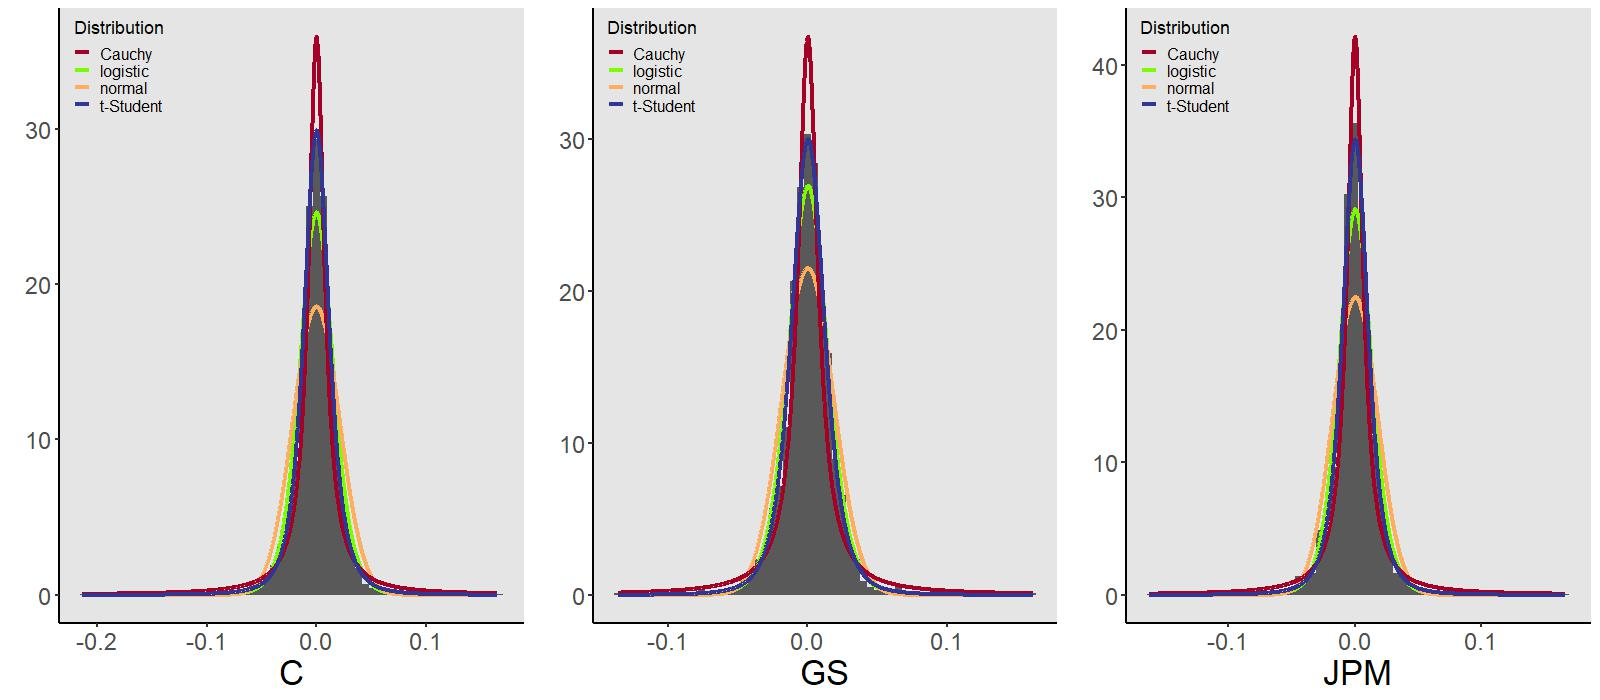
\includegraphics[width=1\textwidth]{figures/marginals/financials_comapnies.jpeg}
\end{figure}
    
\end{frame}

\begin{frame}{Fitted marginals (IT)}

\centering
\begin{figure}[!h]
  \centering
    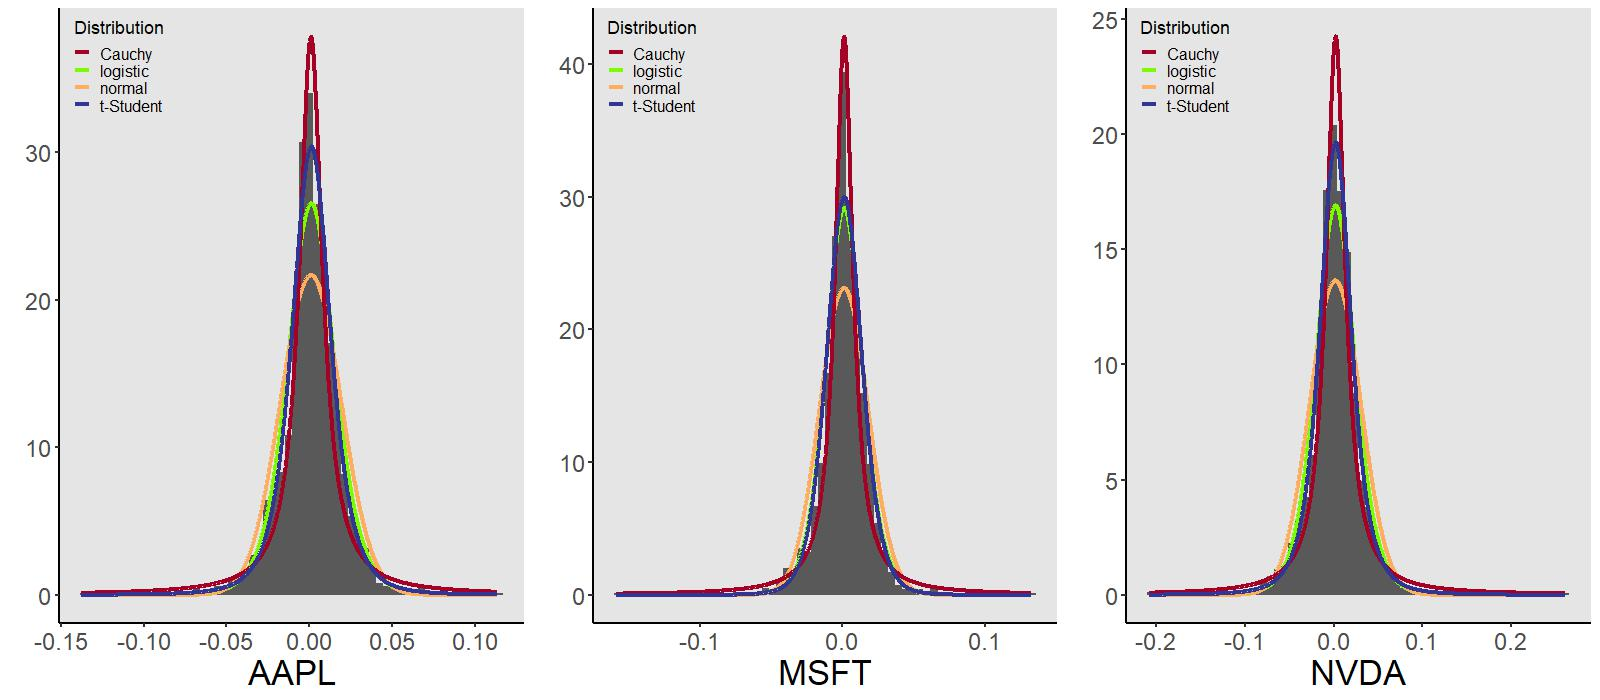
\includegraphics[width=1\textwidth]{figures/marginals/IT_comapnies.jpeg}
\end{figure}
    
\end{frame}

\begin{frame}{Fitted marginals (Services)}

\centering
\begin{figure}[!h]
  \centering
    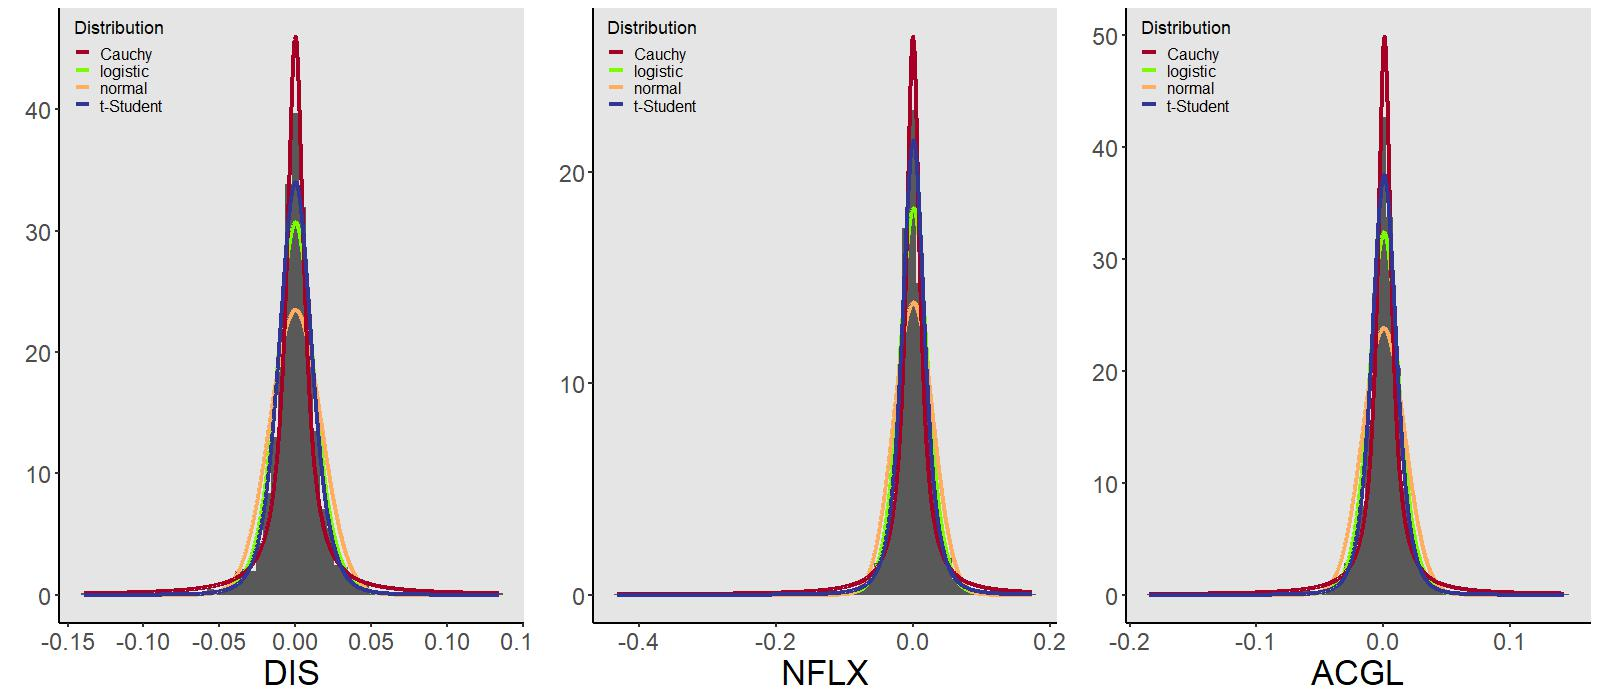
\includegraphics[width=1\textwidth]{figures/marginals/services_comapnies.jpeg}
\end{figure}
    
\end{frame}

\begin{frame}{Elliptical \& Archimedean copulas}

\centering
\begin{table}
\begin{table}[H]

\caption{Criterion scores for fitted elliptical \& archimedean copulas.}
\centering
\fontsize{11}{13}\selectfont
\begin{tabular}[t]{lrrrrr}
\toprule
 & Gaussian & t-Student & Frank & Clayton & Gumbel\\
\midrule
AIC & -11882.96 & -12827.35 & -6234.22 & -6818.93 & -6523.37\\
BIC & -11681.09 & -12619.88 & -6228.61 & -6813.32 & -6517.76\\
Log.likelihood & 5977.48 & 6450.68 & 3118.11 & 3410.47 & 3262.68\\
\bottomrule
\end{tabular}
\end{table}
   
\end{table}

\end{frame}

\begin{frame}{Spearman matrix for fitted t-Student copula}
\centering
\begin{figure}[!h]
  \centering
    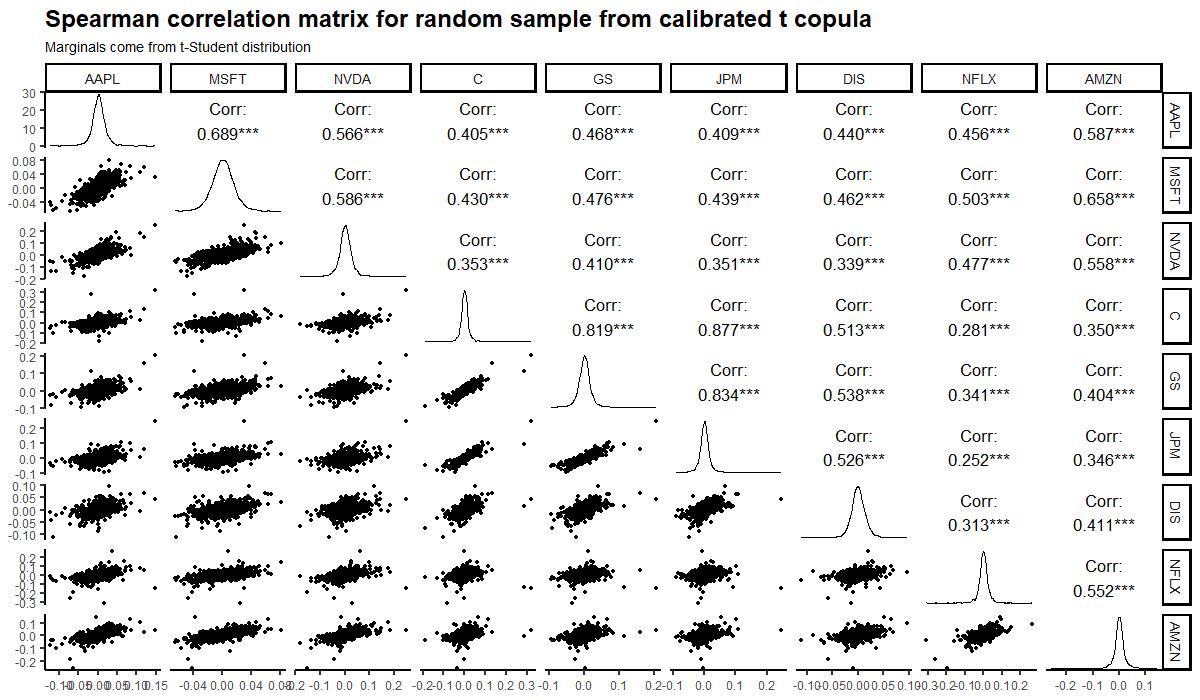
\includegraphics[width=1\textwidth]{figures/correlation/spearman_copula_t_seed_123.jpeg}
\end{figure}
    
\end{frame}

\begin{frame}{Spearman matrix real data vs data sampled from t-Student}
\centering
\begin{figure}[!h]
  \centering
    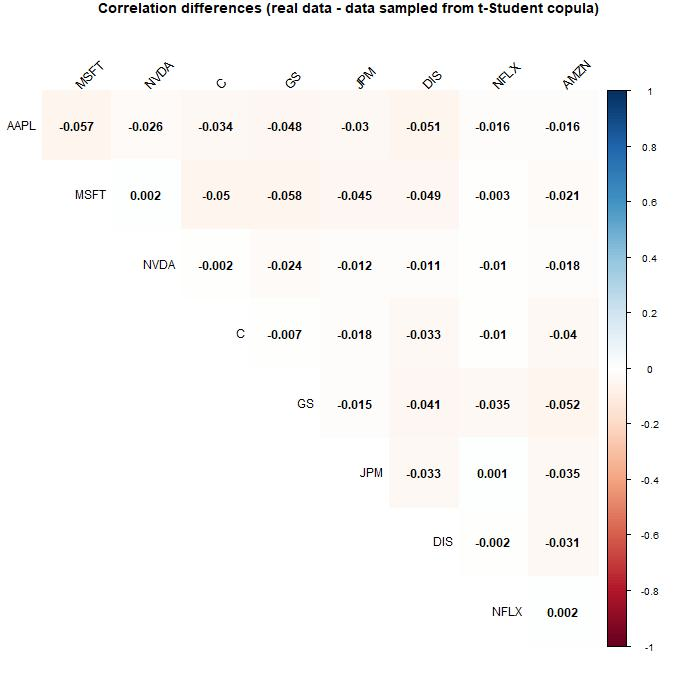
\includegraphics[width=0.7\textwidth]{figures/correlation/spearman_real_data_vs_t_copula.jpeg}
\end{figure}
    
\end{frame}

\begin{frame}{Vines copulas}

\centering
\begin{table}
\begin{table}[H]

\caption{Criterion scores for fitted C-vine, D-vine \& R-vine copulas.}
\centering
\fontsize{11}{13}\selectfont
\begin{tabular}[t]{lrrr}
\toprule
 & D-vine & C-vine & R-vine\\
\midrule
AIC & -13233.54 & -13141.37 & -13219.14\\
BIC & -12925.14 & -12810.54 & -12899.52\\
Log.likelihood & 6671.77 & 6629.69 & 6666.57\\
\bottomrule
\end{tabular}
\end{table}
   
\end{table}

\end{frame}

\begin{frame}{Results for different D-vine structures}

\centering
\begin{table}
% latex table generated in R 4.2.2 by xtable 1.8-4 package
% Tue Sep 26 22:57:45 2023
\begin{tabular}{lr}
  \hline
Structure & Log-likelihood \\ 
  \hline
1,3,2,6,5,4,7,8,9 & 6632.08 \\ 
  9,8,7,6,4,5,2,1,3 & 6646.75 \\ 
  6,5,4,9,7,8,2,3,1 & 6586.13 \\ 
  9,8,7,1,2,3,6,4,5 & 6653.05 \\ 
  7,8,9,2,1,3,4,6,5 & 6662.43 \\ 
  1,3,2,7,8,9,5,4,6 & 6597.40 \\ 
  8,7,9,2,1,3,6,5,4 & 6662.80 \\ 
  4,6,5,7,9,8,1,3,2 & 6594.87 \\ 
  3,1,2,9,7,8,5,4,6 & 6648.26 \\ 
  3,1,2,9,8,7,6,5,4 & 6671.77 \\ 
   \hline
\end{tabular}
   
\end{table}

\end{frame}

\begin{frame}{Vines trees (C-vine, D-vine, R-vine)}

\centering
\begin{figure}[!h]
  \centering
    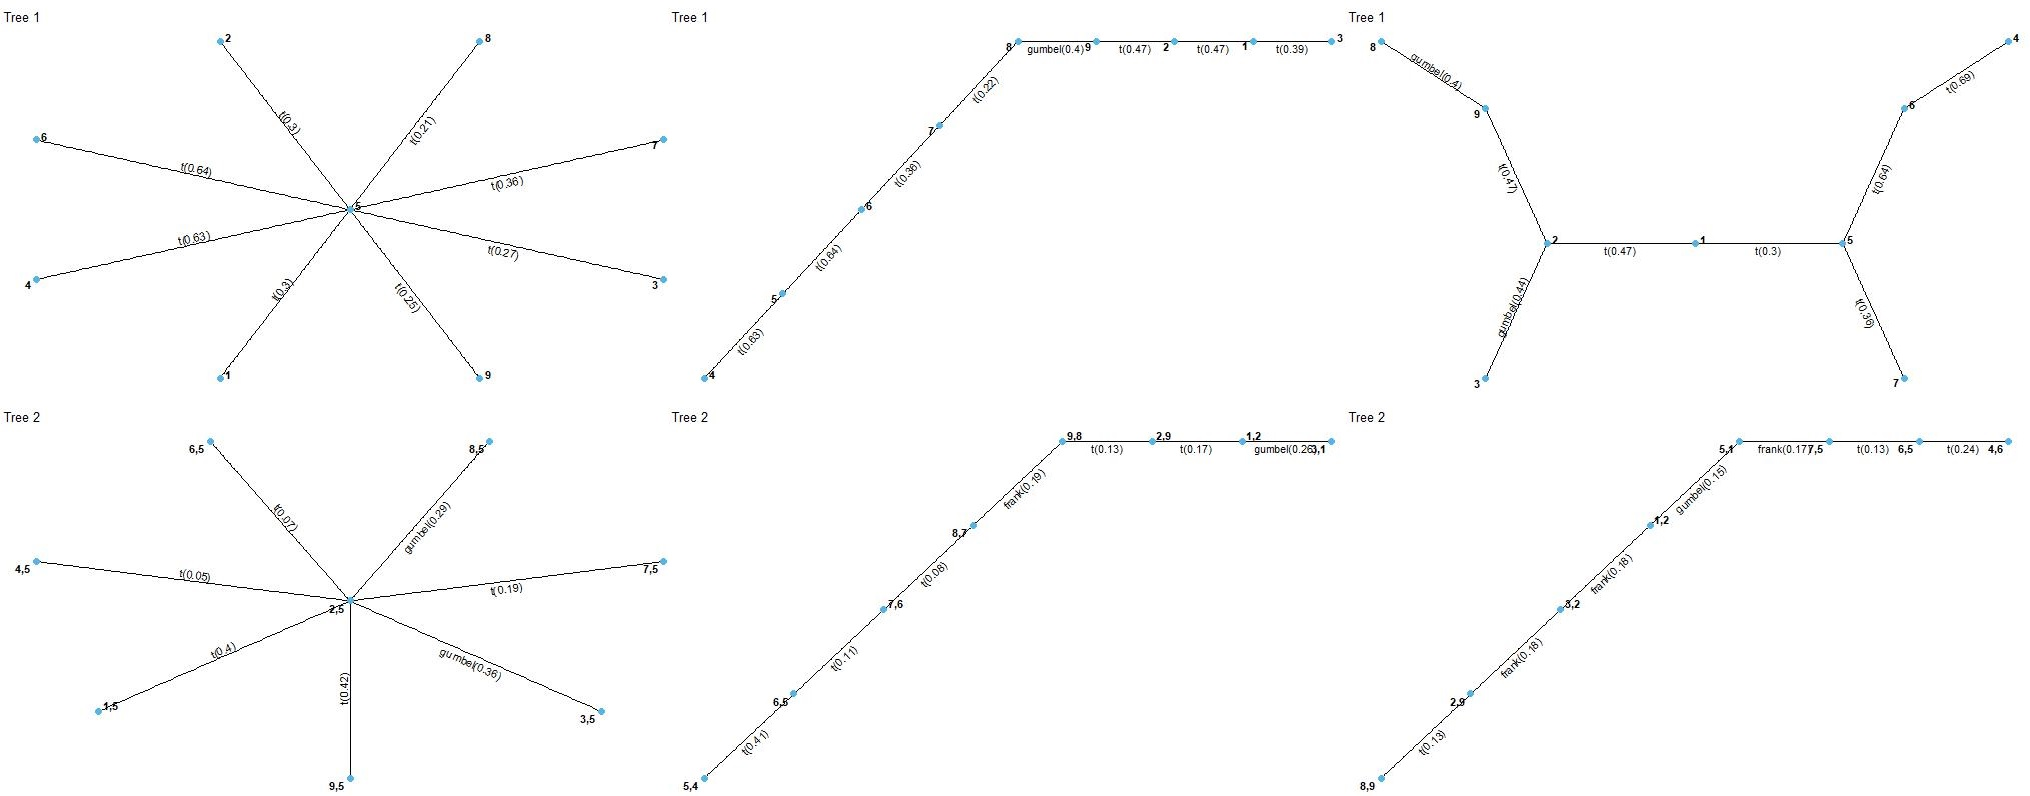
\includegraphics[width=\textwidth]{figures/vine_trees/vine_trees.jpg}
\end{figure}
\end{frame}

\begin{frame}{Spearman matrix for fitted D-vine}
\centering
\begin{figure}[!h]
  \centering
    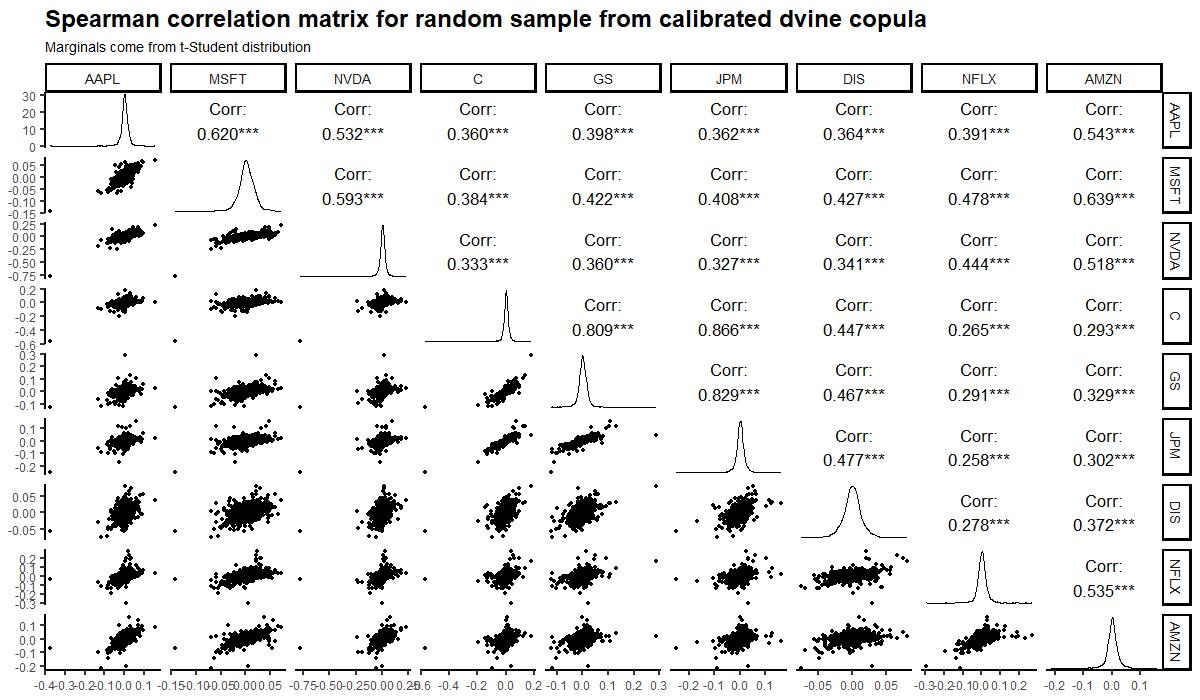
\includegraphics[width=1\textwidth]{figures/correlation/spearman_copula_dvine_seed_123.jpeg}
\end{figure}
    
\end{frame}

\begin{frame}{Spearman matrix real data vs data sampled from D-vine}

\centering
\begin{figure}[!h]
  \centering
    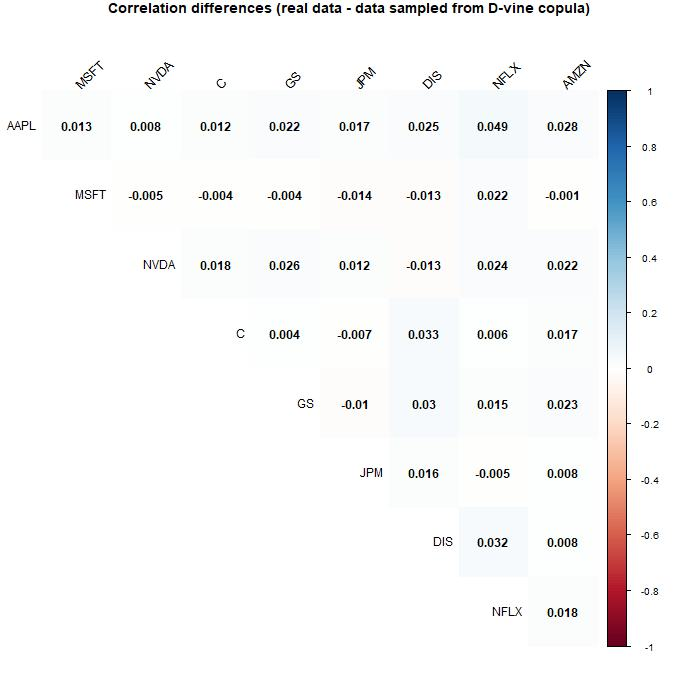
\includegraphics[width=0.7\textwidth]{figures/correlation/spearman_real_data_vs_dvine_copula.jpeg}
\end{figure}
    
\end{frame}

\begin{frame}{Log-likelihood for different bicopula families}

\centering
\begin{table}
\begin{table}[H]

\caption{Log-likelihood scores for fitted vine copulas while variour bicopula families are in usage.}
\centering
\fontsize{11}{13}\selectfont
\begin{tabular}[t]{lrrr}
\toprule
Bicopula family & C-vine & D-vine & R-vine\\
\midrule
all & 7845.96 & 7834.47 & 7848.46\\
parametrics\_except\_tll & 6636.08 & 6674.77 & 6696.81\\
nonparametrics\_indep\_tll & 7845.92 & 7834.45 & 7848.52\\
oneparam & 6324.18 & 6356.26 & 6405.11\\
twoparam & 6636.08 & 6674.77 & 6696.80\\
ellipticals & 6602.22 & 6634.06 & 6635.83\\
arch & 6215.65 & 6238.32 & 6351.13\\
kendalls\_inversion & 6629.69 & 6665.08 & 6666.57\\
kernel\_transform & 7846.26 & 7834.46 & 7848.11\\
epllip\_archimed & 6629.69 & 6665.08 & 6666.57\\
\bottomrule
\end{tabular}
\end{table}
   
\end{table}

\end{frame}

\begin{frame}{Scatter plot $GS \sim DIS$ (D-vine)}

\centering
\begin{figure}[!h]
  \centering
    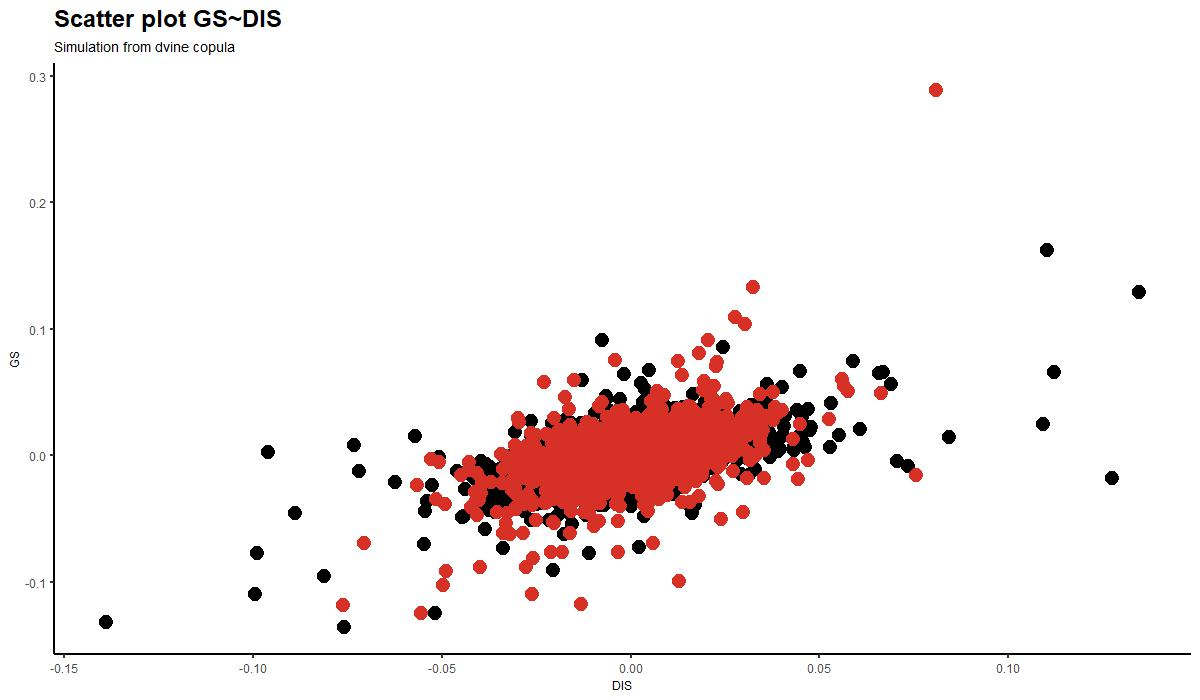
\includegraphics[width=1\textwidth]{figures/GS_vs_DIS/GS_vs_DIS_dvine.jpeg}
\end{figure}
\end{frame}

\begin{frame}{Scatter plots $GS \sim DIS$}

\begin{figure}%
    \centering
    {{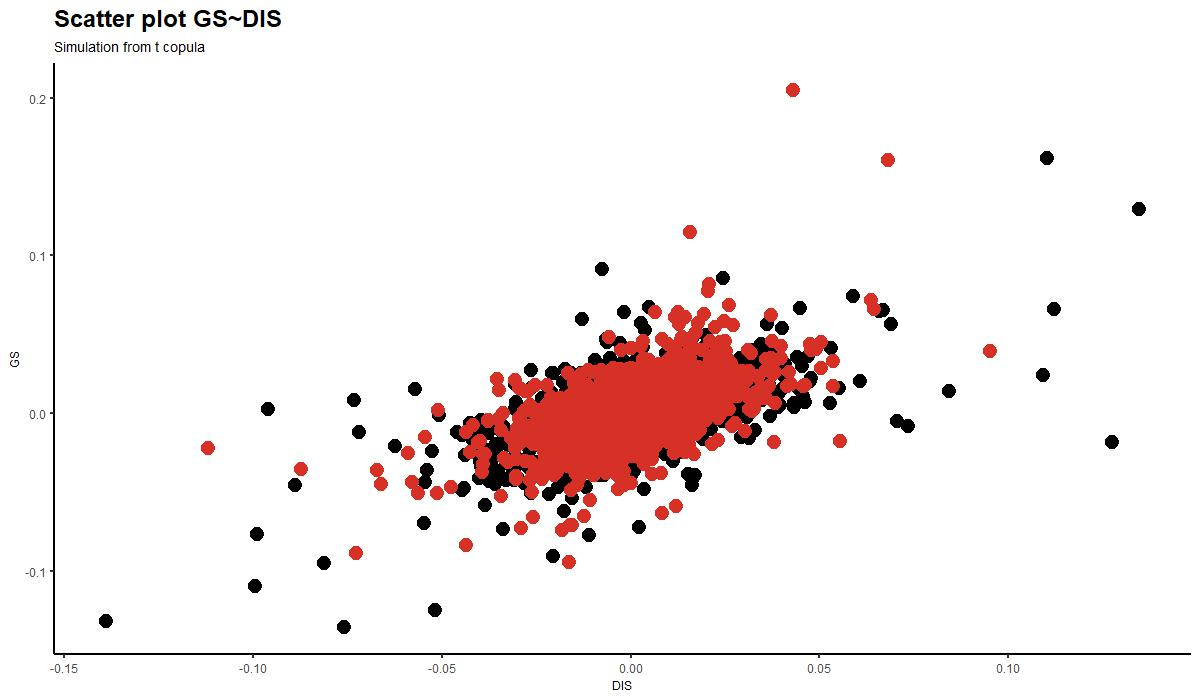
\includegraphics[width=5.3cm]{figures/GS_vs_DIS/GS_vs_DIS_t.jpeg} }}%
    \qquad
    {{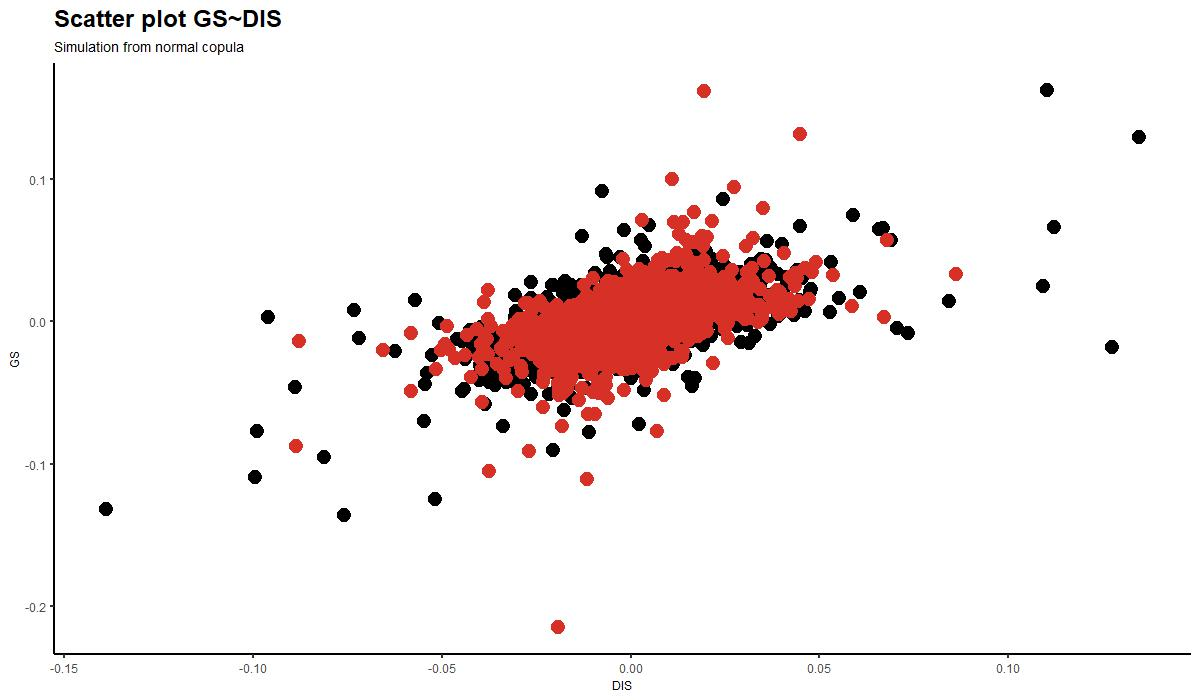
\includegraphics[width=5.3cm]{figures/GS_vs_DIS/GS_vs_DIS_normal.jpeg} }} 
        \centering
    {{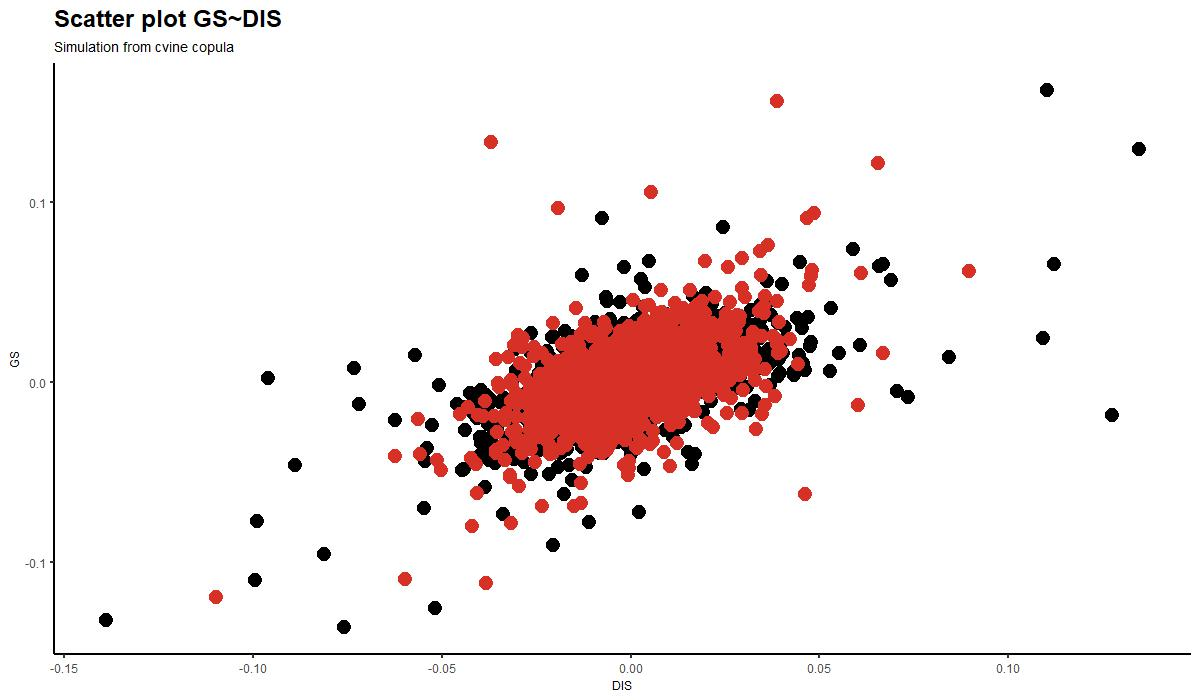
\includegraphics[width=5.3cm]{figures/GS_vs_DIS/GS_vs_DIS_cvine.jpeg} }}%
    \qquad
    {{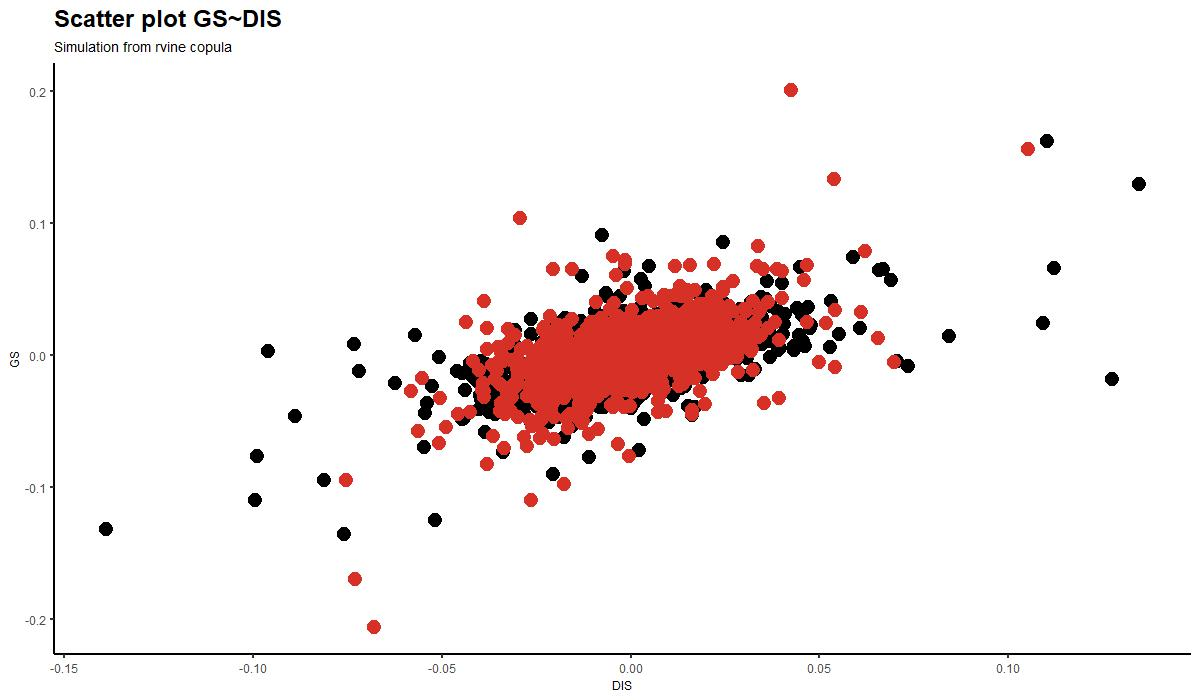
\includegraphics[width=5.3cm]{figures/GS_vs_DIS/GS_vs_DIS_rvine.jpeg} }} 
\end{figure} 
    
\end{frame}

\end{document}